% TA-IND-01 — Análisis del sistema real: App Banco Guayaquil.
% Documento académico con requisitos propuestos, NO resultados de ensayos ejecutados.
\documentclass[conference,a4paper]{IEEEtran}
\usepackage[T1]{fontenc}
\usepackage[utf8]{inputenc}
\usepackage[spanish,es-tabla]{babel}
\usepackage{lmodern,microtype,csquotes,graphicx,booktabs,tabularx,array,xcolor}
\usepackage[backend=biber,style=ieee,sorting=none,maxbibnames=3]{biblatex}
\addbibresource{referencias.bib}
\DeclareFieldFormat{url}{\href{#1}{\texttt{enlace web}}}
\usepackage[hidelinks]{hyperref}
\usepackage{needspace}
\newcolumntype{Y}{>{\raggedright\arraybackslash}X}
\newcommand{\requisito}[3]{\par\noindent\textbf{#1 -- #2.} #3\par\vspace{1pt}}
\setlength{\parindent}{0.75em}
\setlength{\parskip}{1pt}
\renewcommand{\arraystretch}{1.08}
\setlength{\columnsep}{0.24in}
\title{IEEE 29148 y clasificación de requisitos:\\ estudio de la App Banco Guayaquil}
\author{\IEEEauthorblockN{Cedeño Avila Winston Damian}
\IEEEauthorblockA{Universidad Técnica Estatal de Quevedo (UTEQ)\\Ingeniería de Software -- 4.º ``B'' -- ISR-401\\TA-TAR-01 / TA-IND-01 -- 7 de noviembre de 2026}}
\begin{document}
\maketitle
\begin{abstract}
Se estudia la formulación de requisitos verificables con base en ISO/IEC/IEEE 29148:2018 y se aplica a la aplicación móvil de Banco Guayaquil. Se proponen quince requisitos de cinco tipos, se clasifican cinco requisitos de calidad conforme a ISO/IEC 25010:2023 y se realiza una revisión de ambigüedad y criterios de aceptación. Se distinguen las funciones documentadas por el banco de los objetivos técnicos planteados para este ejercicio. Se incluyen tres fotografías propias de la aplicación con información personal y financiera oculta.
\end{abstract}
\section{Sistema elegido y alcance}
La App Banco Guayaquil permite a clientes con credenciales válidas consultar saldos y movimientos, registrar destinatarios, efectuar transferencias y revisar comprobantes. En 2026 el banco comunicó una reorganización de la experiencia de pagos; sus guías diferencian la navegación de Android e iPhone \cite{banco2026,ayudaBG,saldosBG,comproBG}. Este trabajo se centra en los flujos comunes documentados para la \emph{app móvil}, con ejemplos de navegación Android. No se analiza la banca web. El sistema fue escogido para esta actividad; su prioridad de registro en el foro del SGA debe ser confirmada.
\section{Resumen analítico de ISO/IEC/IEEE 29148:2018}
\subsection{De necesidad a requisito}\label{sec:resumen}
La norma empieza por diferenciar una necesidad de su especificación. El usuario puede expresar ``quiero saber si mi dinero llegó'', pero esa frase todavía deja abiertas cuestiones esenciales: qué operación, quién puede consultarla y qué resultado se considera confiable. La cláusula 5.2.3 explica la transformación progresiva de necesidades en requisitos. En la aplicación analizada, conocer el resultado de una transferencia puede convertirse en un enunciado que obliga a mostrar un comprobante solo cuando existe un estado confirmado. Eso permite comprobar posteriormente la decisión, en lugar de depender de la interpretación del desarrollador \cite[cl.~5.2.3]{iso29148}.

La cláusula 5.2.4 describe la construcción del requisito bien formado. Un enunciado debe identificar al sujeto --por ejemplo, la aplicación--, una acción exigible y, cuando corresponde, el evento o condición que activa esa acción. También ha de tener una razón asociada a la necesidad del interesado, restricciones que definan sus límites y una forma posible de verificar el resultado. No se trata de convertir toda preferencia en una obligación. ``Deseo una app cómoda'' es una expectativa; ``antes de confirmar una transferencia, se mostrarán el banco receptor, los cuatro últimos dígitos de la cuenta y el monto'' constituye un comportamiento observable \cite[cl.~5.2.4]{iso29148}.

La diferencia práctica consiste en escribir \emph{qué} resultado se espera, sin obligar prematuramente a una solución técnica. Por ejemplo, exigir que el saldo se consulte mediante un servidor específico limitaría innecesariamente las alternativas de diseño. Es preferible definir la información mostrada y las condiciones de autorización. De acuerdo con Pohl, separar contexto, necesidad y especificación ayuda a detectar decisiones todavía no justificadas y a negociar aspectos pendientes antes de programar \cite{pohl2025}. La norma distingue igualmente requisitos de distintos niveles; un requisito de usuario y otro de componente no llevan la misma cantidad de detalle. Mezclarlos hace difícil decidir quién es responsable de cumplirlos.

\subsection{Las nueve cualidades del requisito individual}
En la cláusula 5.2.5 se exigen nueve cualidades: \emph{necesario, apropiado, no ambiguo, completo, singular, factible, verificable, correcto y conforme}. Necesario significa que su ausencia deja una necesidad sin resolver. Apropiado exige un nivel de detalle adecuado: no se debe imponer arquitectura cuando solo se define un servicio de usuario. No ambiguo permite una interpretación única; completo establece el contexto suficiente para entender el comportamiento sin adivinar información. Singular significa una obligación principal por enunciado, incluso cuando esa obligación tenga varias condiciones \cite[cl.~5.2.5]{iso29148}.

Las otras cuatro cualidades conectan el texto con su aplicación real. Factible plantea que exista una solución técnica y económica razonable; verificable exige una inspección, demostración o prueba capaz de confirmar el resultado; correcto significa representar la necesidad que le dio origen; conforme obliga a seguir el estilo de redacción acordado. En banca móvil, declarar que las consultas tendrán respuesta instantánea sería poco factible y difícil de comprobar. En cambio, especificar un percentil y una carga de ensayo permite discutir un umbral realista y después contrastarlo con mediciones. La cifra, sin embargo, sigue siendo una \emph{meta propuesta}: no se puede atribuir al banco sin haber obtenido sus registros operativos.

\subsection{El conjunto importa tanto como cada enunciado}
La cláusula 5.2.6 añade cinco propiedades del \emph{conjunto}: completo, consistente, factible, comprensible y susceptible de validación. El conjunto debe cubrir las necesidades seleccionadas, evitar contradicciones y usar términos coherentes. Un requisito que confirme pagos y otro que emita comprobantes ante estados pendientes entraría en conflicto aun si cada frase estuviera bien redactada. Por ello, la revisión debe comparar los quince requisitos entre sí, no solo leerlos por separado \cite[cl.~5.2.6]{iso29148}.

La completitud no significa que un ejercicio de quince requisitos represente toda la complejidad de un banco. Aquí solo se cubren flujos delimitados: saldo, movimientos, beneficiarios, transferencias y comprobantes. La consistencia exige la misma denominación de cuenta origen, beneficiario y confirmación en todos los casos. La factibilidad del conjunto implica que las metas de rendimiento y seguridad puedan alcanzarse simultáneamente. Ser comprensible no es sinónimo de escribir menos: significa que otro lector puede relacionar funciones, métricas y criterios sin inventar supuestos. La posibilidad de validación exige cotejar el conjunto con las necesidades de usuarios y responsables del sistema; este paso no se ha realizado con funcionarios del banco.

\subsection{Lenguaje y atributos para evitar errores}
La cláusula 5.2.7 advierte sobre superlativos (``el mejor''), palabras subjetivas (``fácil''), pronombres sin antecedente, adjetivos no medibles (``rápido'', ``mínimo''), expresiones abiertas (``entre otros''), comparaciones sin base y fórmulas evasivas (``cuando sea posible''). También desaconseja absolutos como ``siempre'' y combinaciones lógicas ambiguas. Esta revisión permitió sustituir expresiones como ``seguro'', ``con rapidez'' o ``sin errores nunca'' por condiciones y umbrales comprobables \cite[cl.~5.2.7]{iso29148}.

Los atributos de la cláusula 5.2.8, como identificador, versión, prioridad y justificación, acompañan el requisito pero no sustituyen su contenido \cite[cl.~5.2.8]{iso29148}. Un identificador ayuda a rastrear el cambio, mientras que el criterio de aceptación delimita cómo se comprobaría. SWEBOK v4.0 también trata los requisitos funcionales, las condiciones de calidad y las restricciones como categorías que requieren análisis y acuerdos explícitos \cite{swebok2024}. En síntesis, una especificación útil no consiste en acumular afirmaciones técnicas, sino en poder explicar para qué existe cada una, qué evidencia la sustenta y bajo qué prueba se aceptaría.


\subsection{Aplicar la norma a una aplicación existente}
El caso de la banca móvil muestra por qué un requisito documentado no debe confundirse con una característica observada. La guía del banco permite confirmar, por ejemplo, que existen opciones para consultar cuentas, registrar destinatarios y revisar comprobantes. Pero no expone el contrato de la API, los parámetros reales de carga ni las tasas de disponibilidad del servicio. Por esa razón, los requisitos de interfaz y calidad formulados en este informe están expresados como propuestas de aceptación, no como mediciones ni promesas oficiales. Esta distinción también modifica la forma de redactar: es legítimo proponer que un sistema resista una carga determinada; no es legítimo afirmar que ya la cumple sin contar con un ensayo reproducible.

La elección de tipos de requisito también necesita criterio. Mostrar un saldo o emitir un comprobante corresponde a un comportamiento funcional observable. Recibir la respuesta de un servicio bancario se estudia como interfaz externa, porque necesita un intercambio de datos con otro sistema. Verificar el saldo antes de iniciar una transferencia describe una regla de proceso. Ofrecer información relevante antes de pulsar la confirmación pertenece a los factores humanos y al uso de la interfaz. Finalmente, fijar segundos, porcentajes, tasas de rechazo o interpretación de mensajes define propiedades de calidad. La misma necesidad general de ``transferir dinero'' no autoriza a escribir quince frases equivalentes: exige identificar obligaciones distintas y evitar contradicciones entre sus condiciones.

Una precaución adicional surge de las diferencias entre versiones de la aplicación. Banco Guayaquil ha comunicado modificaciones en su interfaz y sus instrucciones públicas distinguen rutas de Android e iPhone \cite{banco2026,ayudaBG}. Un requisito referido a una pantalla concreta podría dejar de ser adecuado después de una actualización, aunque la necesidad del cliente siga vigente. Por eso, cuando es posible, se describe la información y el comportamiento esperado en vez de imponer el nombre de un botón de una versión. Aun así, para verificar una función concreta será necesario identificar la versión, dispositivo y fecha de las capturas. Este punto conecta la claridad del requisito individual con la consistencia del conjunto, como proponen las cláusulas 5.2.5 y 5.2.6 \cite[cl.~5.2.5--5.2.6]{iso29148}.

La autoevaluación no debe convertirse en una tabla que marque automáticamente ``cumple'' a todo. Aspectos como singularidad o claridad pueden examinarse leyendo el enunciado, pero la necesidad real y la factibilidad técnica requieren contrastarlo con quienes conocen el producto y sus restricciones. Para este ejercicio se proponen revisiones de escritorio, criterios y pruebas futuras; la aprobación operativa del banco queda fuera del alcance. Reconocer ese límite hace más defendible la propuesta que atribuir una certeza que la evidencia disponible no permite sostener.

\section{Glosario de diez términos (cláusula 3)}
\noindent\textbf{1. Requisito (cl. 3.1.19).} Enunciado que convierte una necesidad en una condición exigible del sistema. \emph{Ejemplo:} Mostrar un comprobante tras una transferencia confirmada.

\noindent\textbf{2. Stakeholder (cl. 3.1.28).} Interesado que usa o se ve afectado por el producto. \emph{Ejemplo:} El cliente y el operador bancario tienen necesidades diferentes.

\noindent\textbf{3. Condición (cl. 3.1.6).} Circunstancia que determina cuándo se aplica una obligación. \emph{Ejemplo:} Después de autenticarse, se consulta el saldo.

\noindent\textbf{4. Restricción (cl. 3.1.7).} Límite impuesto a la solución o su operación. \emph{Ejemplo:} Solo cuentas autorizadas pueden mostrar información privada.

\noindent\textbf{5. Requisito derivado (cl. 3.1.10).} Obligación inferida de otros requisitos o de una solución adoptada. \emph{Ejemplo:} Del control de acceso se deriva impedir consultar cuentas ajenas.

\noindent\textbf{6. Elicitación (cl. 3.1.20).} Obtención estructurada de las necesidades de quienes intervienen. \emph{Ejemplo:} Observar cómo un usuario busca un comprobante.

\noindent\textbf{7. Trazabilidad (cl. 3.1.23).} Relación que permite seguir el origen y el destino de un requisito. \emph{Ejemplo:} Vincular RF-04 con la necesidad de conservar constancia de pago.

\noindent\textbf{8. Matriz de trazabilidad (cl. 3.1.24).} Tabla que conecta requisitos con necesidades o elementos de prueba. \emph{Ejemplo:} Relacionar RC-11 con la prueba de tiempo de consulta.

\noindent\textbf{9. Validación de requisitos (cl. 3.1.25).} Revisión para saber si la especificación responde a las necesidades correctas. \emph{Ejemplo:} Comprobar con usuarios si el resumen previo evita errores.

\noindent\textbf{10. Verificación de requisitos (cl. 3.1.26).} Examen de claridad y buena formulación de los enunciados. \emph{Ejemplo:} Revisar si RC-12 tiene período y porcentaje precisos.

\section{Quince requisitos propuestos}\label{sec:req}
Los enunciados siguientes constituyen \emph{una especificación académica propuesta}, no una descripción interna certificada del producto. Las funciones observables se contrastaron con las guías del banco \cite{ayudaBG,saldosBG,comproBG}; los procesos, interfaces y umbrales se proponen para evaluación.
\requisito{RF-01}{Consulta de saldo}{Tras autenticar al cliente, la aplicación deberá mostrar el saldo disponible en USD de la cuenta que este seleccione, expresado con dos decimales.}
\requisito{RF-02}{Movimientos recientes}{Cuando el cliente seleccione una cuenta, la aplicación deberá mostrar una lista ordenada por fecha descendente con los últimos diez movimientos existentes de esa cuenta, incluyendo fecha, concepto e importe.}
\requisito{RF-03}{Registro de beneficiario}{Cuando el cliente registre un beneficiario de transferencia, la aplicación deberá guardar el banco receptor, el número de cuenta y el nombre del beneficiario únicamente después de validar los campos obligatorios.}
\requisito{RF-04}{Comprobante de transferencia}{Después de una transferencia confirmada, la aplicación deberá mostrar un comprobante con identificador de operación, fecha, importe y estado que el cliente pueda compartir.}
\requisito{IE-05}{Resultado de transferencia}{Cuando el servicio bancario responda a una solicitud de transferencia, la aplicación deberá interpretar el identificador, importe y estado de la operación según el contrato de integración aprobado.}
\requisito{IE-06}{Código de verificación}{Cuando la entidad requiera una verificación adicional, la aplicación deberá solicitar al servicio de autenticación autorizado un código de un solo uso destinado al canal registrado del cliente.}
\requisito{PR-07}{Validación previa a transferir}{Antes de transmitir una orden de transferencia, la aplicación deberá validar que el importe solicitado sea mayor que USD 0,00 y no exceda el saldo disponible de la cuenta origen.}
\requisito{PR-08}{Prevención de doble envío}{Si una transferencia ya tiene un identificador en estado pendiente, la aplicación deberá impedir que una segunda pulsación de confirmación genere otra solicitud con el mismo identificador.}
\requisito{US-09}{Ingreso de monto}{En el formulario de transferencia, la aplicación deberá informar que el importe es inválido cuando el cliente introduzca un valor no numérico o un importe con más de dos decimales.}
\requisito{US-10}{Resumen antes de confirmar}{Antes de que el cliente confirme una transferencia, la aplicación deberá presentar en una misma pantalla el banco de destino, los últimos cuatro dígitos de la cuenta receptora y el importe en USD.}
\requisito{RC-11}{Tiempo de consulta}{Con 150 sesiones de ensayo simultáneas durante veinte minutos, el percentil 95 del tiempo de respuesta de la consulta de saldo deberá ser de 2,5 segundos o menos.}
\requisito{RC-12}{Disponibilidad de consultas}{Durante treinta días de observación, al menos el 99,5 \% de las sondas programadas cada minuto al servicio de consulta de saldo deberá completarse correctamente.}
\requisito{RC-13}{Confidencialidad del saldo}{En una batería de 120 solicitudes de ensayo sin sesión válida o sobre cuentas ajenas, la aplicación deberá impedir la exposición del saldo y los movimientos protegidos en 120 de 120 casos.}
\requisito{RC-14}{Prevención de errores del usuario}{Al presentar una cuenta receptora distinta de la seleccionada previamente, al menos 18 de 20 participantes de ensayo deberán detectar la diferencia en el resumen de transferencia antes de confirmar, sin ayuda.}
\requisito{RC-15}{Interoperabilidad de confirmaciones}{En una batería de sesenta mensajes válidos de confirmación definidos por el contrato de la interfaz de transferencias, la aplicación deberá interpretar correctamente sesenta de sesenta identificadores, importes y estados.}

\section{Clasificación, métrica y aceptación}\label{sec:tabla}
La clasificación conserva cinco tipos (funcional, interfaz externa, proceso, usabilidad/factor humano y calidad). Para RC-11 a RC-15 se usa \emph{característica / subcaracterística} de ISO/IEC 25010:2023; se evita confundir la métrica propuesta con un resultado medido \cite{iso25010}.
\begin{table*}[!t]
\centering\caption{Clasificación y criterios de aceptación de los quince requisitos}
\fontsize{7.1}{8.3}\selectfont
\begin{tabularx}{\textwidth}{@{}p{0.75cm}p{4.0cm}p{1.55cm}p{3.4cm}Y@{}}
\toprule ID & Enunciado y acción exigida & Tipo & ISO 25010 / métrica & Criterio de aceptación \\
\midrule
RF-01 & Mostrar saldo disponible de la cuenta elegida tras autenticación. & Funcional & No aplica / prueba funcional & Cuenta autorizada con saldo simulado de USD 42,30: mostrar 42,30 y no saldos de otra cuenta. \\
RF-02 & Mostrar los diez movimientos recientes de una cuenta en orden de fecha. & Funcional & No aplica / prueba funcional & Cuenta con doce movimientos de prueba: presentar diez, en orden descendente. \\
RF-03 & Registrar un beneficiario después de validar los datos exigidos. & Funcional & No aplica / prueba funcional & Con cuenta incompleta: rechazar registro; con datos válidos: guardar un beneficiario. \\
RF-04 & Mostrar comprobante compartible de una transferencia confirmada. & Funcional & No aplica / prueba funcional & Operación confirmada: comprobante con cuatro campos y opción de compartir; rechazada: sin comprobante de éxito. \\
IE-05 & Interpretar respuesta del servicio de transferencias según el contrato. & Interfaz & No aplica / prueba funcional & Simular respuestas aprobada, rechazada y pendiente: cada una debe mostrar el estado correspondiente. \\
IE-06 & Solicitar código de un solo uso al servicio de verificación autorizado. & Interfaz & No aplica / prueba funcional & Servicio de ensayo: una petición válida genera solicitud al destino registrado; canal no registrado: rechazo. \\
PR-07 & Validar saldo e importe antes de enviar la transferencia. & Proceso & No aplica / prueba funcional & Importes -1,00, 0,00 y mayor al saldo: impedir la orden; importe permitido: continuar. \\
PR-08 & Impedir dos envíos del mismo identificador de orden pendiente. & Proceso & No aplica / prueba funcional & Dos pulsaciones consecutivas de una orden pendiente: emitir una sola solicitud de ensayo. \\
US-09 & Avisar si el importe contiene caracteres o decimales inválidos. & Usabilidad & No aplica / prueba funcional & Valores abc y 2,345: mostrar aviso antes de confirmar; 2,34: permitir continuar. \\
US-10 & Mostrar banco, últimos cuatro dígitos e importe antes de confirmar. & Usabilidad & No aplica / prueba funcional & Escenario de ensayo: comprobar que los tres datos aparecen antes del botón final. \\
RC-11 & Responder consultas de saldo con p95 no mayor de 2,5 segundos. & Calidad & Eficiencia desempeño / comportamiento temporal / p95 (s) & Prueba de carga: p95 <= 2,5 s para consultas correctas con 150 sesiones, veinte minutos. \\
RC-12 & Cumplir el porcentaje mínimo de sondas correctas durante 30 días. & Calidad & Fiabilidad / disponibilidad / éxito (\%) & Éxitos/sondas previstas * 100 >= 99,5 \% en treinta días; incluir fallos del servicio. \\
RC-13 & Impedir exposición del saldo ante 120 accesos no autorizados. & Calidad & Seguridad / confidencialidad / 120 intentos & Rechazar 120 intentos no autorizados sin divulgar campos protegidos en respuesta ni pantalla. \\
RC-14 & Lograr detección de error de destino por 18 de 20 usuarios. & Calidad & Capacidad de interacción / protección de errores / 18 de 20 & Ensayo de usabilidad: 18/20 (90 \%) identifican el cambio antes de confirmar. \\
RC-15 & Interpretar 60 mensajes válidos del servicio de transferencias. & Calidad & Compatibilidad / interoperabilidad / 60 de 60 & Prueba de contrato: 60/60 mensajes válidos interpretados sin errores. \\
\bottomrule
\end{tabularx}
\end{table*}

\section{Autoevaluación y corrección (15 de 15)}
La siguiente revisión documental contrasta enunciados iniciales con las nueve propiedades de la cláusula 5.2.5: necesidad (N), adecuación (A), no ambigüedad (U), completitud (C), singularidad (S), factibilidad (F), verificabilidad (V), corrección (Co) y conformidad (Cf). Además se buscaron las expresiones de 5.2.7. Se mantienen la versión previa y su corrección en dos tablas; los textos finales también aparecen en la sección~\ref{sec:req}. El análisis no representa pruebas de funcionamiento.
\begin{table*}[!t]
\centering\caption{Autoevaluación: versión original, diagnóstico y corrección (1/2)}
\fontsize{7.4}{8.6}\selectfont
\begin{tabularx}{\textwidth}{@{}p{0.70cm}p{3.45cm}p{3.45cm}Y@{}}
\toprule ID & Versión original & Diagnóstico de 5.2.5 y 5.2.7 & Versión corregida \\
\midrule
RF-01 & La app mostrará el saldo rápidamente. & Se cambió «rápidamente» por un dato verificable de saldo y formato. & Tras autenticar al cliente, la aplicación deberá mostrar el saldo disponible en USD de la cuenta que este seleccione, expresado con dos decimales. \\
RF-02 & La aplicación enseñará todos los movimientos. & Se delimitó el alcance a diez registros y el orden de presentación. & Cuando el cliente seleccione una cuenta, la aplicación deberá mostrar una lista ordenada por fecha descendente con los últimos diez movimientos existentes de esa cuenta, incluyendo fecha, concepto e importe. \\
RF-03 & El cliente podrá guardar contactos fácilmente. & Se reemplazó un juicio subjetivo por campos y condiciones de aceptación. & Cuando el cliente registre un beneficiario de transferencia, la aplicación deberá guardar el banco receptor, el número de cuenta y el nombre del beneficiario únicamente después de validar los campos obligatorios. \\
RF-04 & La app siempre dará un buen comprobante. & Se precisaron contenido y condición; se evitó «siempre» y «buen». & Después de una transferencia confirmada, la aplicación deberá mostrar un comprobante con identificador de operación, fecha, importe y estado que el cliente pueda compartir. \\
IE-05 & La app se conectará bien con el banco. & Se definieron datos observables y estados de respuesta; contrato aún no conocido. & Cuando el servicio bancario responda a una solicitud de transferencia, la aplicación deberá interpretar el identificador, importe y estado de la operación según el contrato de integración aprobado. \\
IE-06 & El sistema enviará códigos cuando sea necesario. & Se identificó el evento y el destino; es un comportamiento propuesto, no API confirmada. & Cuando la entidad requiera una verificación adicional, la aplicación deberá solicitar al servicio de autenticación autorizado un código de un solo uso destinado al canal registrado del cliente. \\
PR-07 & La aplicación revisará que el dinero esté bien. & Se fijaron límites de valor y condición de proceso. & Antes de transmitir una orden de transferencia, la aplicación deberá validar que el importe solicitado sea mayor que USD 0,00 y no exceda el saldo disponible de la cuenta origen. \\
PR-08 & La aplicación evitará transacciones duplicadas en lo posible. & Se eliminó «en lo posible» y se acotó el evento repetido. & Si una transferencia ya tiene un identificador en estado pendiente, la aplicación deberá impedir que una segunda pulsación de confirmación genere otra solicitud con el mismo identificador. \\
\bottomrule
\end{tabularx}
\end{table*}
\begin{table*}[!t]
\centering\caption{Autoevaluación: versión original, diagnóstico y corrección (2/2)}
\fontsize{7.4}{8.6}\selectfont
\begin{tabularx}{\textwidth}{@{}p{0.70cm}p{3.45cm}p{3.45cm}Y@{}}
\toprule ID & Versión original & Diagnóstico de 5.2.5 y 5.2.7 & Versión corregida \\
\midrule
US-09 & La pantalla será intuitiva para todos. & Se sustituyó «intuitiva» por errores de entrada reproducibles. & En el formulario de transferencia, la aplicación deberá informar que el importe es inválido cuando el cliente introduzca un valor no numérico o un importe con más de dos decimales. \\
US-10 & La aplicación permitirá confirmar con toda la información necesaria. & Se especificaron tres datos concretos y un momento de presentación. & Antes de que el cliente confirme una transferencia, la aplicación deberá presentar en una misma pantalla el banco de destino, los últimos cuatro dígitos de la cuenta receptora y el importe en USD. \\
RC-11 & La app será muy rápida. & Se fijaron carga, unidad, duración, percentil y umbral. & Con 150 sesiones de ensayo simultáneas durante veinte minutos, el percentil 95 del tiempo de respuesta de la consulta de saldo deberá ser de 2,5 segundos o menos. \\
RC-12 & La banca móvil siempre estará disponible. & Se reemplazó «siempre» por porcentaje, ventana y definición de éxito. & Durante treinta días de observación, al menos el 99,5 \% de las sondas programadas cada minuto al servicio de consulta de saldo deberá completarse correctamente. \\
RC-13 & Nadie podrá ver información privada nunca. & Se acotó el conjunto de pruebas y se quitó la promesa absoluta. & En una batería de 120 solicitudes de ensayo sin sesión válida o sobre cuentas ajenas, la aplicación deberá impedir la exposición del saldo y los movimientos protegidos en 120 de 120 casos. \\
RC-14 & Todos los clientes identificarán los errores con facilidad. & Se definieron tarea, participantes y mínimo medible. & Al presentar una cuenta receptora distinta de la seleccionada previamente, al menos 18 de 20 participantes de ensayo deberán detectar la diferencia en el resumen de transferencia antes de confirmar, sin ayuda. \\
RC-15 & La app trabajará perfectamente con otras plataformas. & Se acotaron interfaz, datos y tasa de aceptación. & En una batería de sesenta mensajes válidos de confirmación definidos por el contrato de la interfaz de transferencias, la aplicación deberá interpretar correctamente sesenta de sesenta identificadores, importes y estados. \\
\bottomrule
\end{tabularx}
\end{table*}
\noindent\textit{Síntesis de las nueve cualidades:} el análisis de la redacción comprueba adecuación, ausencia de ambigüedad, completitud, singularidad, verificabilidad y conformidad formal. La necesidad real, factibilidad y correspondencia con las expectativas del banco no se pueden dar por validadas mediante documentos públicos; requieren participación del titular del producto y de sus responsables técnicos. Esta limitación es común a los quince enunciados corregidos.

\clearpage
\section{Evidencia visual del sistema real}\label{sec:figuras}
La Figura~\ref{fig:evidencias} reúne tres fotografías propias de la versión Android de la aplicación. Antes de incorporarlas se ocultaron datos de personas y operaciones; únicamente se utilizan para acreditar opciones visibles, no resultados de pruebas de seguridad o rendimiento \cite{ayudaBG,banco2026}.
\par\medskip\noindent
\begin{center}
\begin{minipage}[t]{0.31\columnwidth}\centering
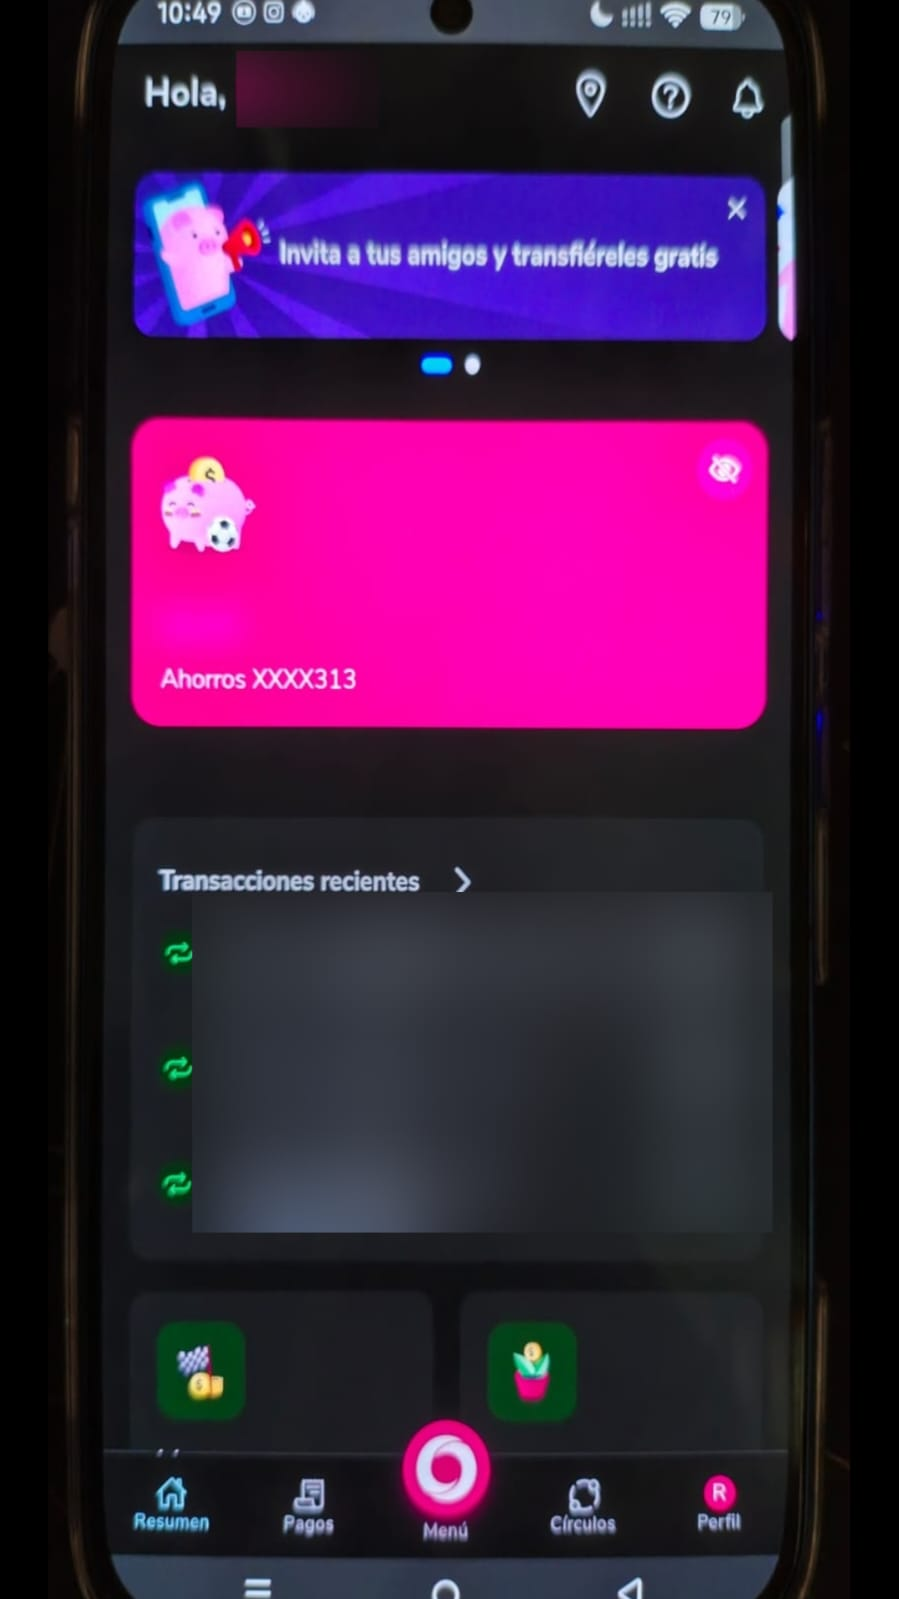
\includegraphics[height=3.3cm,keepaspectratio]{figuras/figura_01_inicio.jpg}\par
{\scriptsize (a) Inicio y resumen}\end{minipage}\hfill
\begin{minipage}[t]{0.31\columnwidth}\centering
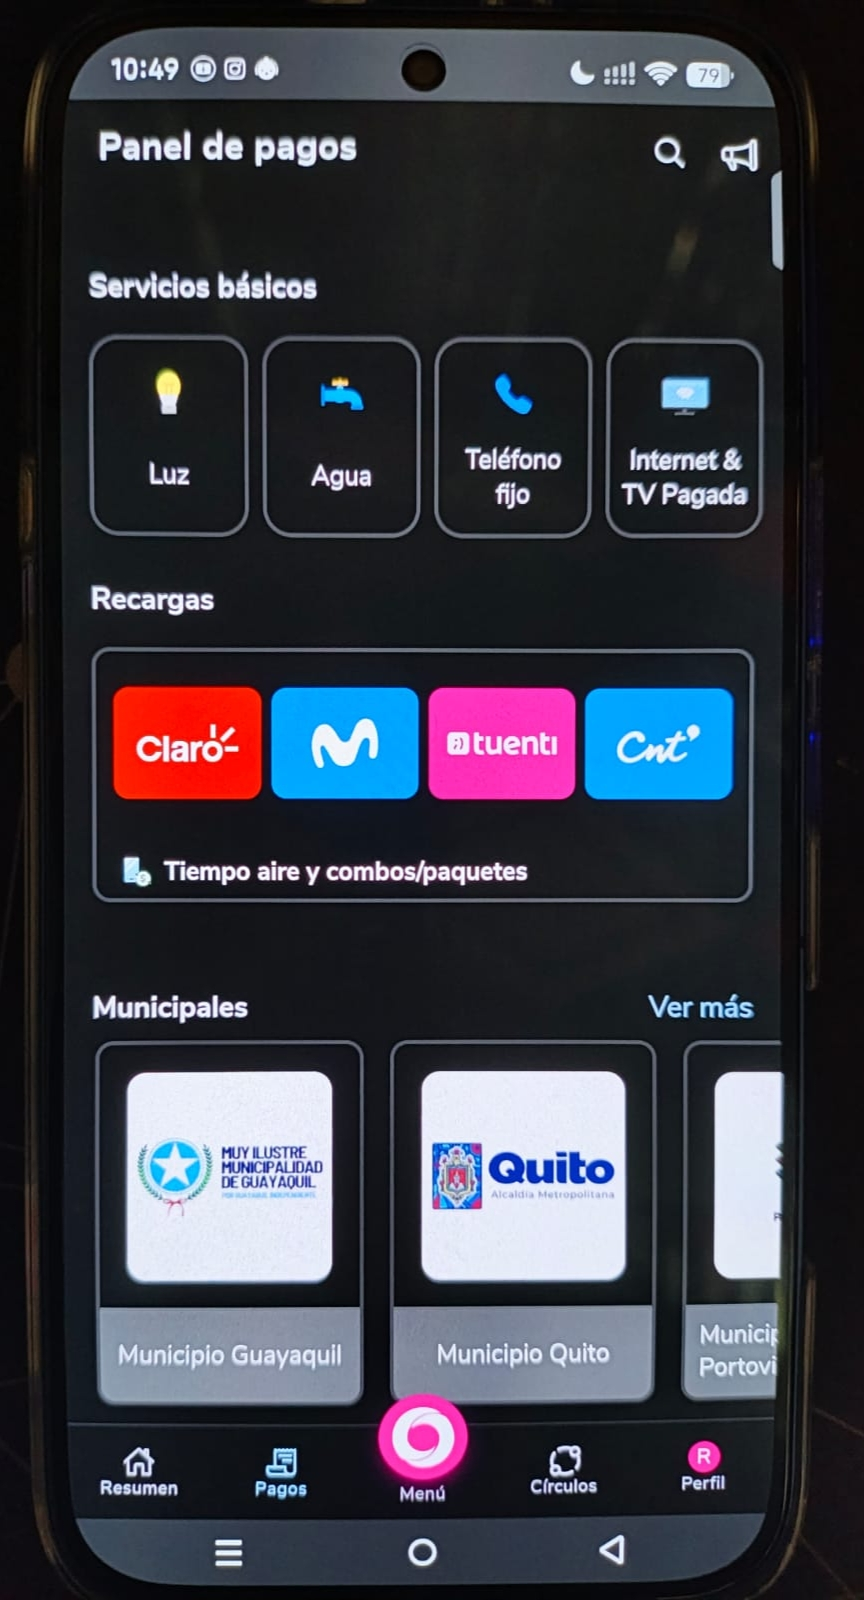
\includegraphics[height=3.3cm,keepaspectratio]{figuras/figura_02_pagos.jpg}\par
{\scriptsize (b) Panel de pagos}\end{minipage}\hfill
\begin{minipage}[t]{0.31\columnwidth}\centering
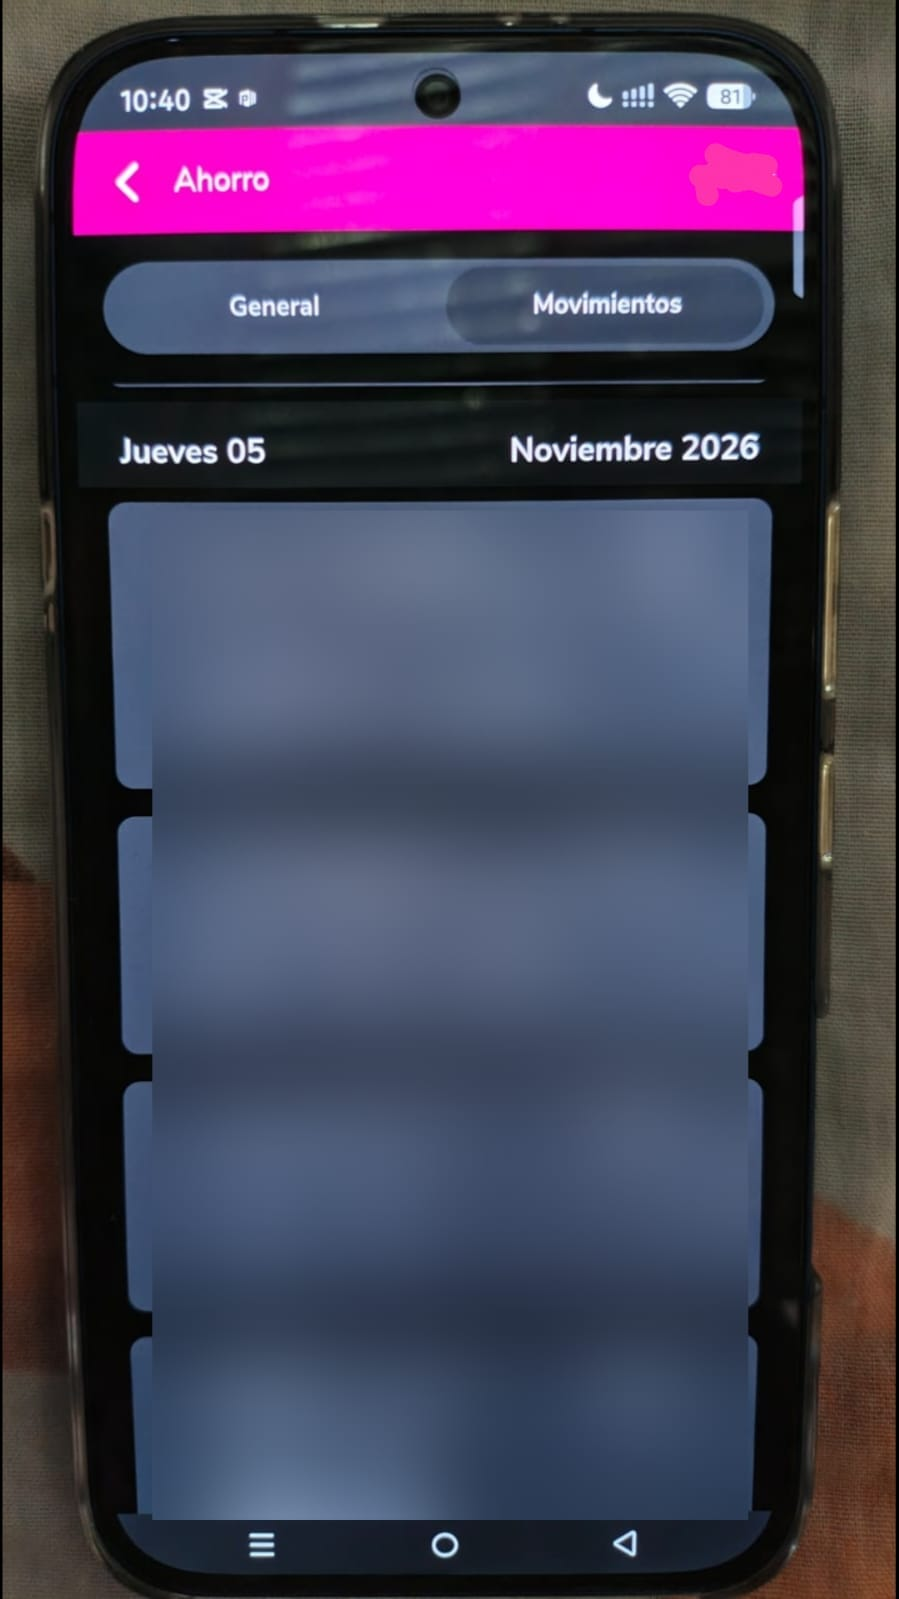
\includegraphics[height=3.3cm,keepaspectratio]{figuras/figura_03_movimientos.jpg}\par
{\scriptsize (c) Movimientos}\end{minipage}
\par\smallskip\refstepcounter{figure}\label{fig:evidencias}
{\footnotesize\textbf{Figura~\thefigure.} Fotografías propias: inicio, pagos e historial de movimientos. Datos sensibles ocultos.}
\end{center}
\medskip

\section{Reflexión crítica sobre la formulación}\label{sec:reflex}
La mayor dificultad de esta propuesta aparece al pasar de una función visible a una condición de calidad: observar que una aplicación permite transferir dinero no demuestra cuánto tarda cada operación, qué porcentaje de disponibilidad alcanza ni cómo valida sus solicitudes internas. Es necesario distinguir tres clases de información: hechos observables en la interfaz, explicaciones públicas del banco y metas definidas exclusivamente para un ejercicio académico. Confundirlas lleva a inventar pruebas o a presentar hipótesis como resultados. La norma ayuda precisamente a separar estos niveles.

Una segunda dificultad surge cuando una frase intenta reunir demasiados comportamientos. Por ejemplo, ``transferir, avisar y emitir comprobante rápidamente'' parece una sola necesidad, pero contiene varias obligaciones y una palabra ambigua. Dividirla en requisitos independientes permite comprobar cada resultado y localizar el origen de un fallo. También se aprendió que un porcentaje, por sí solo, no basta: debe indicarse la población de ensayo, la duración, el método y la condición de aceptación. El mismo 95\% puede significar cosas distintas si se mide sobre diez consultas o sobre miles de operaciones concurrentes.

La revisión también muestra límites que no deben ocultarse. El contrato de los servicios internos del Banco Guayaquil no es público para esta actividad, de modo que los requisitos de interfaz se plantean como hipótesis. Las capturas incorporadas respaldan opciones visibles de la app, pero no prueban la seguridad o el rendimiento de los servicios bancarios. Una etapa posterior tendría que validar estas propuestas con usuarios y responsables autorizados. El aprendizaje principal es formular compromisos verificables sin confundir la experiencia del cliente con supuestos sobre la implementación.

\section*{Referencias}
\printbibliography[heading=none]
\noindent\footnotesize\textbf{Declaración de IA.} Se utilizó ChatGPT (OpenAI, GPT-6, noviembre de 2026) como apoyo para organizar la estructura en LaTeX, generar propuestas de redacción y revisar expresiones ambiguas. Se contrastaron los títulos y cláusulas citadas con fuentes disponibles de ISO/IEEE y las funciones de la aplicación con publicaciones oficiales de Banco Guayaquil. Los requisitos y umbrales constituyen propuestas académicas: no se realizaron entrevistas ni pruebas sobre la infraestructura del banco. Las fotografías propias se incorporaron como evidencias visuales con datos sensibles ocultos; su contenido debe interpretarse únicamente como observación de interfaz.
\end{document}
